\section{Styrenhet}
Styrenhetens uppgift är att styra motorerna utifrån data som skickas från kommunikationsenheten.
Styrenheten ska kunna vara i två lägen, autonomt läge då den reglerar motorerna utifrån sensorvärden eller 
fjärrstyrt läge då den tar emot och behandlar styrkommandon.
\subsection{Hårdvara}
Styrmoodulen består av en AVR ATmega16 som ska placeras på robotplattformen.
Mikroprocessorns PWM-utgångar ska kopplas till PWM-ingångarna på robotplattformen för att styra motorerna.
För att styra riktning på motorerna kopplas två I/O-utgångar från mikroprocessorn till plattformens riktningsingångar.
\subsection{Mjukvara}
Mjukvaran kommer att fungera väldigt olika beroende på om roboten är i fjärrstyrt eller autonomt läge.
\subsubsection{Fjärrstyrt läge}
I fjärrstyrt läge så genereras ett avbrott när ett kommando tagits emot.
Varje kommando är en byte långt där de fyra mest signifikanta bitarna bestämmer vilket kommando som ska utföras
och de 4 minst signifikanta bitarna bestämmer hur kommandot ska utföras (t ex hur snabbt roboten ska svänga).
Uppdelningen kan ses i tabell \ref{styrbitar}.

\begin{table}[h] 
        \label{styrbitar}
        \begin{center}
                \begin{tabular}{| c | c |}
                        \hline
                        Kommando [4 bitar] & Hastighet [4 bitar] \\ \hline
                \end{tabular}
        \end{center}
        \caption{Bituppdelning av styrkommandon}
\end{table}
I avbrottsrutinen så tolkas kommandot och PWM-utgångarna och I/O-utgångarna som styr riktningarna på motorerna ställs.
Så om inget nytt avbrott kommer så fortsätter det senaste kommandot.
Kodningen av kommandon ses i tabell \ref{kodning}.

\begin{table}[h] 
        \label{kodning}
        \begin{tabular}{l l}
                \textbf{4 MSB} & \textbf{Kommando} \\
                0000 & Stopp \\
                0001 & Framåt \\
                0010 & Fram vänster \\
                0011 & Fram höger \\
                0100 & Rotera vänster \\
                0101 & Rotera höger \\
                0110 & Back \\
        \end{tabular}
        \caption{Kommandokodning}
\end{table}

\subsubsection{Autonomt läge}
I autonomt läge så ska styrenheten ta emot skillnaden mellan aktuella och önskade sensorvärden och styra motorerna utifrån detta.
För att undvika att roboten slingrar sig fram när den följer linjer eller väggar så kommer en PD-regulator att användas, se \ref{reglering}.
När data har tagits emot så genereras ett avbrott. I avbrottsrutinen kommer själva regleringen att ske. Datat som tas emot är en byte långt 
och tolkas som ett signat heltal. Utöver den vanliga regleringen ska fyra specialkommandon kunna hanteras, sväng vänster 90\degree, sväng höger 90\degree
, kör rakt fram och återuppta vanlig reglering.

\subsection{Reglering}
\label{reglering}
En PD-regulator kommer att användas för att undvika att roboten slingrar sig fram och för att ett litet stationärt fel inte kommer att störa
den autonoma styrningen mycket. I figur \ref{regulator} ses ett blockschema på regulatorn där r är referenssignalen,
e är felet (skillnaden mellan aktuellt och önskat läge), u är insignalen (hur motorerna styrs) och y är utsignalen (robotens position).
Formeln för PD-reglering är: $$ u[n] = K_P*e[n] + K_D\frac{e[n]-e[n-1]}{\Delta T}$$
Där konstanterna $K_P$, $K_D$ och $\Delta T$ ska bestämmas. $K_P$ är konstanten som styr den proportionella delen (P) av regleringen, 
$K_D$ är konstanten som styr den deriverande delen (D) av regleringen och $\Delta T$ är tiden mellan två sensoravläsningar. 
För att bestämma konstanterna måste mätningar göras på sensorer, motorer och roboten.

\begin{figure}[H]
        \label{regulator}
        \begin{center}
                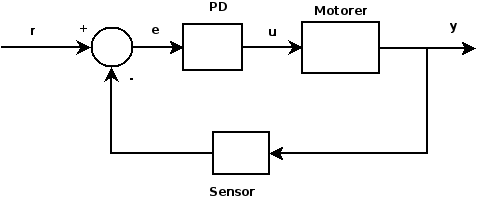
\includegraphics[scale=0.7]{bilder/regulator.png}
        \end{center}
        \caption{Regulatorns blockschema}
\end{figure}

\subsection{Blockschema}
Se appendix \ref{app:styrenhet}
